\documentclass{article} % For LaTeX2e
\usepackage{iclr2027_conference,times}

% Optional math commands from https://github.com/goodfeli/dlbook_notation.
\input{math_commands.tex}

\usepackage{url}
\usepackage{microtype}
\usepackage{graphicx}
\usepackage{booktabs} % for professional tables
\usepackage{pdfpages}
\usepackage{caption}
\usepackage{tabularx}
\usepackage{subcaption}
\usepackage{booktabs} 
\usepackage{longtable}
\usepackage{pdflscape}
\usepackage{algorithm}
\usepackage{algorithmicx}
\usepackage{algpseudocode}
\usepackage{amsmath}
\usepackage{amssymb}
\usepackage{mathtools}
\usepackage{amsthm}
\usepackage{color} 
\usepackage{amsfonts}
\usepackage{booktabs}
\usepackage{xtab}
\usepackage{afterpage}
\usepackage{booktabs}
\usepackage{multirow}
\usepackage{caption}
\usepackage{wrapfig}
\usepackage{enumitem}
\usepackage{subcaption}
% Keep the draft table compilable with minimal TinyTeX installations.
\IfFileExists{colortbl.sty}{\usepackage{colortbl}}{\newcommand{\rowcolor}[1]{}}
\usepackage[T1]{fontenc}
\usepackage[hypcap=false]{caption}


\title{On the Pitfalls of Verbalized Confidence Priors for Calibrating Reasoning LLMs}

% Authors must not appear in the submitted version. They should be hidden
% as long as the \iclrfinalcopy macro remains commented out below.
% Non-anonymous submissions will be rejected without review.

\author{
    % authors
  Shuoyuan Wang\textsuperscript{1},\enspace
  Yixuan Li\textsuperscript{2},\enspace
  Hongxin Wei \textsuperscript{1 }\thanks{Correspond to \texttt{weihx@sustech.edu.cn}.}, \enspace \\
  \textsuperscript{1}Department of Statistics and Data Science, Southern University of Science and Technology  \\
  \textsuperscript{2}Department of Computer Sciences, University of Wisconsin-Madison\\
%   \texttt{\{\}@smail.nju.edu.cn},\enspace chjwang@nju.edu.cn,\enspace weihx@sustech.edu.cn \\
  % \texttt{huangjg@shanghaitech.edu.cn, 12112806@sustech.edu.cn,}\\
  % \texttt{linjun.zhang@rutgers.edu, huaxiu@cs.unc.edu} \\
}


\definecolor{mydarkred}{rgb}{0.6,0,0}
\definecolor{mydarkgreen}{rgb}{0,0.6,0}
\definecolor{calibrow}{gray}{0.94}
\newcommand{\fix}{\marginpar{FIX}}
\newcommand{\new}{\marginpar{NEW}}

\newtheorem{theorem}{Theorem}
\newtheorem{lemma}{Lemma}
\newtheorem{proposition}{Proposition}
\newtheorem{definition}{Definition}
\renewcommand\arraystretch{1.2}

% for draft 
\newcommand{\red}[1]{\textcolor{red}{#1}}
\newcommand{\blue}[1]{\textcolor{blue}{#1}}
\usepackage[colorlinks,
linkcolor=mydarkred,
citecolor=mydarkgreen]{hyperref}


\begin{document}


\maketitle

\begin{abstract}
The abstract paragraph should be indented 1/2~inch (3~picas) on both left and qaqqa

\end{abstract}

\section{Introduction}

Reasoning large language models (LLMs) increasingly solve complex problems by generating a reasoning trajectory followed by the answer~\citep{yang2025qwen3}. 
Despite these advances, the answer accuracy alone does not ensure reliable uncertainty estimates: a model may produce plausible reasoning trajectory yet remain overconfident in an incorrect answer~\citep{geng2024survey, liu2025uncertainty}. 
In principle, confidence calibration requires the reported confidence to reflect the empirical probability that the answer is correct, which in turn enables applications such as hallucination detection \citep{wu2026mitigating} and adaptive test-time scaling \citep{yang2026scaling}.

Verbalized confidence obtains such an answer-level score by asking the model to emit a numerical probability with its final answer. Unlike confidence estimators based on token probabilities, hidden states, or repeated sampling~\citep{luo2026your,srey2026signals,wang2026calibrating}, it can be produced in a single black-box generation~\citep{xiong2024can}. Recent work trains this output with supervised fine-tuning (SFT), using targets derived from correctness or rollout statistics~\citep{lin2022teaching,li2025conftuner}, and with reinforcement learning (RL), by adding calibration terms to answer rewards~\citep{xu2024sayself,damani2026beyond,ma2026decoupling,yang2026scaling}.

We identify one primary failure and one recipe-dependent optimization effect. Under a fixed prompt, format, and decoding protocol, the base model's sampled confidence is concentrated on a small set of values and only moderately stratifies correct and incorrect rollouts. The resulting confidence prior provides limited support for learning a graded correctness estimate. In filtering ablations, completed no-filtering DCPO and RLCR runs further concentrate confidence on a few values and endpoints, whereas the corresponding DAPO-filtered runs retain broader support. We therefore treat confidence concentration as a property of the sampling recipe, rather than as an inevitable consequence of GRPO.

We address the initialization problem with CalibSFT. CalibSFT constructs a target for each rollout by combining the success rate of its prompt group with the rollout's verified correctness. Its selective segment loss retains confidence supervision on incorrect rollouts while restricting reasoning/answer supervision to correct rollouts, and target-balanced sampling exposes the model to a broader range of confidence values. In the subsequent RL stage, all compared methods use the same DAPO-style mixed-outcome filtering~\citep{yu2025dapo} as a fixed sampling recipe, allowing us to compare Base and CalibSFT initialization under controlled downstream optimization.

We make three contributions:
\begin{itemize}[leftmargin=*]
    \item We characterize a concentrated base-model confidence prior and document how confidence concentration depends on the RL sampling recipe.
    \item We introduce CalibSFT, which combines rollout-derived targets, target-balanced sampling, and correctness-aware segment supervision for confidence initialization.
    \item We evaluate whether the CalibSFT initialization improves accuracy, calibration, and confidence diversity after downstream RL across multiple confidence-aware objectives.
\end{itemize}

\section{Preliminaries}

\subsection{Verbalized Confidence for Reasoning LLMs}

In this work, we study confidence calibration for reasoning language models that
verbalize a numerical confidence score~\citep{tian2023just,
xiong2024can}. Given a question $x$, the LLM is tasked with producing a
completion $o=(r,a,c)$, where $r$ is a reasoning trace and $a$ is an answer.
$c\in[0,1]$ is a post-answer confidence value and represents the
model's estimated probability that $a$ is correct.

\paragraph{Reinforcement Learning with Verifiable Rewards (RLVR).}
RLVR formulates the LLM as a policy
$\pi_\theta$ parameterized by $\theta$. Given a question $x$, the policy generates
a rollout $o$, and a task verifier assigns it a binary correctness label
$z=V(x,a)\in\{0,1\}$. Typically, the policy is optimized using Group Relative
Policy Optimization (GRPO)~\citep{shao2024deepseekmath}. In practice, GRPO samples $G$
rollouts $\{o_i\}_{i=1}^{G}$ for each question, and the optimization objective
can then be formulated as:
\begin{equation}
\begin{split}
J_{\mathrm{GRPO}}(\theta)=\mathbb E\Bigg[\frac{1}{G}\sum_{i=1}^{G}
\frac{1}{L_i}\sum_{t=1}^{L_i}\min\Big(&\rho_{i,t}(\theta)\widehat A_i, \operatorname{clip}\!\left(\rho_{i,t}(\theta),1-\epsilon_{\mathrm{clip}},
1+\epsilon_{\mathrm{clip}}\right)\widehat A_i\Big)\Bigg].
\end{split}
\end{equation}
Here $o_i=(o_{i,1},\ldots,o_{i,L_i})$, and
$\rho_{i,t}(\theta)=\pi_\theta(o_{i,t}\mid x,o_{i,<t})/
\pi_{\theta_{\mathrm{old}}}(o_{i,t}\mid x,o_{i,<t})$ is the policy ratio;
$\epsilon_{\mathrm{clip}}$ is the clipping parameter. Given the reward
$R_i=R(o_i)$ and a small constant $\epsilon>0$ for numerical stability, the
group-relative advantage is:
\begin{equation}
    \widehat A_i=\frac{R_i-\bar R}{\sigma_R+\epsilon},\qquad
    \bar R=\frac{1}{G}\sum_{j=1}^{G}R_j,\qquad
    \sigma_R=\operatorname{std}\!\left(\{R_j\}_{j=1}^{G}\right).
\end{equation}

\paragraph{Confidence-Aware Rewards.}
For verbalized confidence training, a confidence-based scoring term is typically
added to the reward. For example, RLCR~\citep{damani2026beyond} adds the negative
Brier loss to the binary correctness reward:
\begin{equation}
    R_i=z_i-(c_i-z_i)^2,
\end{equation}
where $c_i$ denotes the reported confidence and
$z_i=V(x,a_i)\in\{0,1\}$ denotes the correctness label of rollout $i$.
This reward favors correct answers while assigning higher scores to confidence
values that better match their correctness labels, thereby increasing their
probability under GRPO.

\subsection{Calibration Metrics}

A useful verbalized confidence score should be both calibrated and
discriminative~\citep{eusebi2026reading}. To formalize calibration, let $C$ and
$Z$ denote the confidence and correctness random variables, respectively. A
perfectly calibrated score satisfies $\Pr(Z=1\mid C=p)=p$ for every
$p\in[0,1]$. 
To quantify the degree of miscalibration, \textbf{Expected Calibration Error
(ECE)}~\citep{guo2017calibration} is defined as
$\mathbb E_C[|\Pr(Z=1\mid C)-C|]$. In practice, after partitioning $N$
examples into $B$ confidence bins $\{\mathcal I_b\}_{b=1}^{B}$, we estimate
ECE as
\begin{equation}
    \operatorname{ECE}
    =\sum_{b=1}^{B}\frac{|\mathcal I_b|}{N}
    \left|\operatorname{acc}(\mathcal I_b)-
    \operatorname{conf}(\mathcal I_b)\right|.
\end{equation}
Here, $\operatorname{acc}(\mathcal I_b)$ and
$\operatorname{conf}(\mathcal I_b)$ are the mean correctness and confidence in
bin $b$, respectively.
While ECE measures calibration at the bin level, the \textbf{Brier
score}~\citep{brier1950verification} measures the squared error between confidence
and correctness for each instance,
\begin{equation}
    \operatorname{Brier}=\frac{1}{N}\sum_{j=1}^{N}(c_j-z_j)^2,
\end{equation}
where lower values indicate better probabilistic predictions for both metrics.
These metrics assess calibration, but neither directly evaluates discrimination
as a ranking property. For example, assigning every response a constant confidence
equal to the overall accuracy yields zero ECE while giving correct and incorrect
responses identical scores~\citep{eusebi2026reading}. We therefore measure
the discrimination using \textbf{AUROC}, which evaluates whether correct responses receive
higher confidence than incorrect ones.

\section{Motivation}
\label{sec:motivation}

Confidence-aware RL typically optimizes calibration rewards on responses sampled
from LLMs~\citep{damani2026beyond}.
To investigate whether LLMs can learn calibrated confidence estimates through RL,
we analyze how their confidence distributions change during training.

\paragraph{Confidence priors concentrate on a few high values.}
We refer to the confidence distribution before RL as the model's
\emph{confidence prior}.
To characterize this prior, we sample 10 rollouts per question from
Qwen3-8B~\citep{yang2025qwen3},
Gemma4-E2B-Instruct~\citep{team2026gemma},
OLMo3-7B-Instruct~\citep{olmo2025olmo3} on DeepScaleR-Train, and present their confidence distributions in Figure~\ref{fig:initial_confidence_prior}.
All three models concentrate their confidence on a few high values, with fewer than 5\% of outputs below 0.5.
These base models also assign high confidence even to incorrect responses,
suggesting that their verbalized confidence does not reliably reflect
answer correctness.
As a result, RL starts from a sub-optimal confidence prior that rarely produces
low-confidence samples.

\begin{figure}[t]
    \centering
    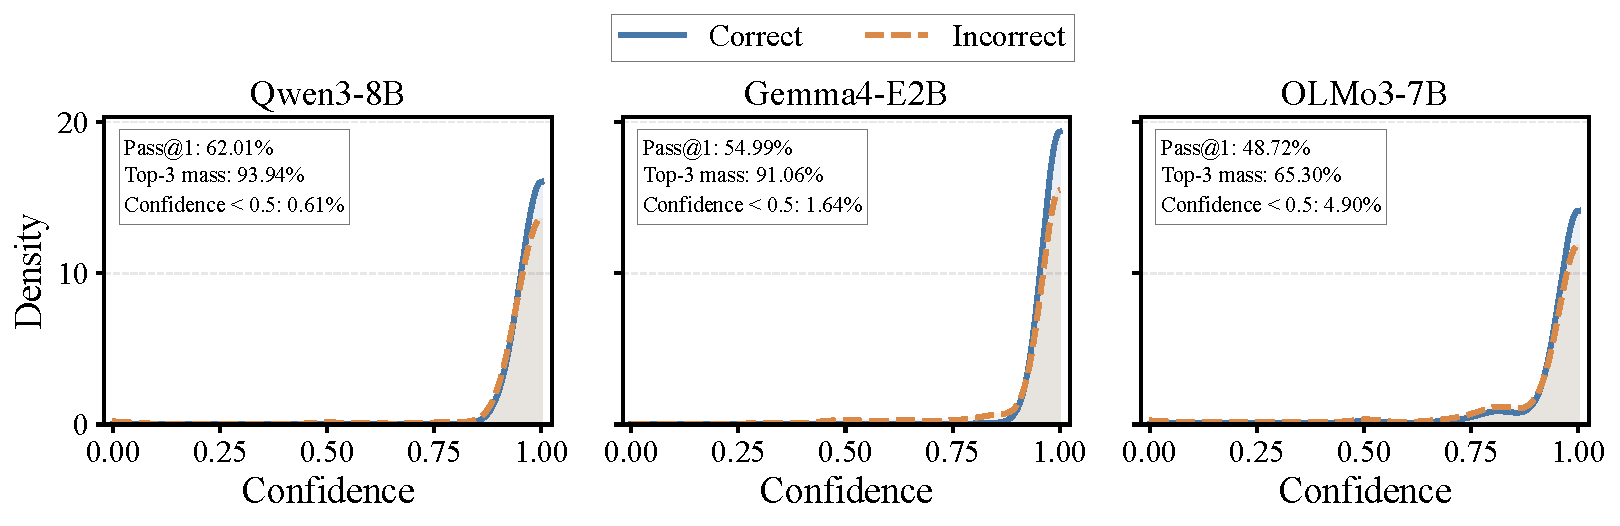
\includegraphics[width=\linewidth]{figures/raw_training_confidence_priors_k10.pdf}
    \caption{Confidence distributions of three representative open-source
    LLMs on DeepScaleR. All three models concentrate probability mass near 1.
    Fewer than 5\% of outputs have confidence below 0.5 for each model.}
    \label{fig:initial_confidence_prior}
\end{figure}

\paragraph{RL improves calibration but confidence exploration remains limited.}
To examine whether calibration-aware RL overcomes this concentration,
we train Qwen3-8B with RLCR.
As shown in Figure~\ref{fig:rlcr_training_calibration}(a), RLCR successfully reduces Brier loss during training, demonstrating its
effectiveness in improving calibration.
However, Figure~\ref{fig:rlcr_training_calibration}(b) shows that
the model continues to sample a small set of confidence values
for each question.
We provide more detailed empirical evidence in
Appendix~\ref{sec:motivation_training_statistics}.

\begin{figure}[t]
    \centering
    \begin{minipage}[t]{0.60\linewidth}
        \vspace{0pt}
        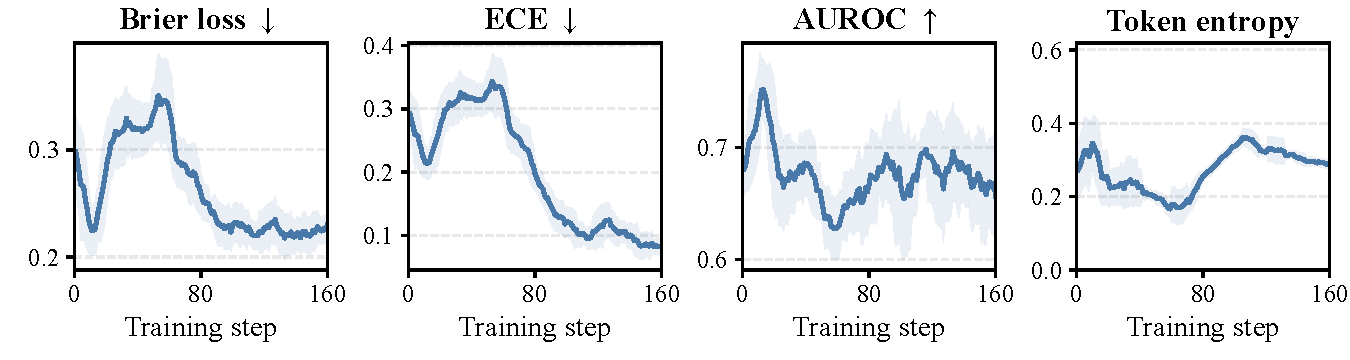
\includegraphics[width=\linewidth]{figures/rlcr_motivation.pdf}
        \caption{Training dynamics of Qwen3-8B with RLCR.
        (a) Brier loss. (b) Distinct confidence values per question
        (eight rollouts; blue, left axis) and confidence token entropy
        (orange, right axis). Bold curves show centered five-step moving
        averages; faint curves show per-step measurements.}
        \label{fig:rlcr_training_calibration}
    \end{minipage}\hfill
    \begin{minipage}[t]{0.38\linewidth}
        \vspace{0pt}
        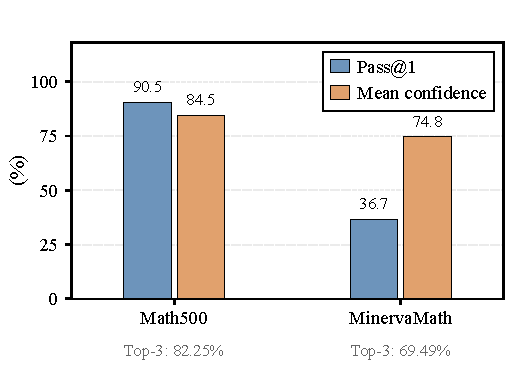
\includegraphics[width=\linewidth]{figures/rlcr_test_calibration.pdf}
        \caption{Test-time calibration at step 160 on Math500 and
        MinervaMath (ID), using four rollouts per question. Bars show Pass@1
        and mean confidence; task labels report Top-3 mass.}
        \label{fig:rlcr_test_calibration}
    \end{minipage}
\end{figure}

To better understand why this concentration persists during training,
we formulate confidence generation as action selection under a softmax
policy and examine how sampling probabilities affect the expected
gradient~\citep{garg2022alternate}.
\begin{proposition}[Policy gradients under confidence concentration]
\label{prop:confidence_saturation}
Fix prediction information $h$ and a finite set of confidence actions
$\{c_1,\ldots,c_K\}\subseteq[0,1]$.
Let $\pi_i=\Pr(C=c_i\mid h)=\exp(\ell_i)/\sum_{j=1}^K\exp(\ell_j)$.
For $Z\in\{0,1\}$ indicating answer correctness, define the fixed
expected reward $r_i=-\mathbb E[(c_i-Z)^2\mid h]$.
Let $J_h(\ell)=\sum_i\pi_i r_i$ and
$\Delta_h=\max_i r_i-\min_i r_i$. Then
\begin{equation}
    \frac{\partial J_h}{\partial\ell_i}=\pi_i(r_i-J_h),
    \qquad
    \left|\frac{\partial J_h}{\partial\ell_i}\right|
    \leq\pi_i\Delta_h.
\end{equation}
If $\pi_k=1-\varepsilon$ for some $k\in\{1,\ldots,K\}$, then
\begin{equation}
    \|\nabla_\ell J_h\|_1\leq 2\varepsilon\Delta_h.
\end{equation}
\end{proposition}
Proposition~\ref{prop:confidence_saturation} shows that a rarely sampled
confidence value has a small expected logit gradient even when choosing it
would improve the expected reward. As the confidence distribution approaches
a single choice, the entire logit gradient vanishes, including when that
choice is suboptimal.
This provides a mechanism by which an initially concentrated confidence
distribution can impede exploration of better-calibrated outputs.
We provide the proof in Appendix~\ref{sec:confidence_saturation_proof}.

\paragraph{Persistent confidence concentration hinders downstream calibration.}
To examine the implications of persistent confidence concentration
for downstream calibration, we evaluate the final RLCR checkpoint
on two datasets of contrasting difficulty including Math500 and MinervaMath.
As shown in Figure~\ref{fig:rlcr_test_calibration}, the post-RL model
underestimates its accuracy on Math500 but is markedly overconfident
on MinervaMath.
Despite the large accuracy gap, the mean confidence remains similar
across the two tasks, with the three most frequent values accounting
for about 70\% of outputs on each tasks.
This suggests that confidence estimates do not sufficiently adapt
to differences in task difficulty, and further contribute to downstream miscalibration.

To characterize the calibration cost of this mismatch, we examine
the expected Brier loss, which is minimized when confidence equals
the conditional probability of correctness~\citep{gneiting2007strictly,damani2026beyond}.
The following proposition quantifies how little probability mass near
this optimal confidence raises the lower bound on Brier loss.
\begin{proposition}[Brier risk under limited confidence sampling]
\label{prop:confidence_support}
Let $Z\in\{0,1\}$ indicate answer correctness and let $C\in[0,1]$
denote the predicted confidence.
Given prediction information $h$, define
$p_h=\Pr(Z=1\mid h)$.
Assume that $C$ and $Z$ are conditionally independent given $h$.
For any $\delta>0$, let
$m_\delta(h)=\Pr(|C-p_h|<\delta\mid h)$.
Then
\begin{equation}
    \mathbb E[(C-Z)^2\mid h]
    \geq p_h(1-p_h)+\delta^2\bigl(1-m_\delta(h)\bigr).
\end{equation}
\end{proposition}
For a fixed neighborhood of $p_h$, Proposition~\ref{prop:confidence_support}
shows that the lower bound on Brier loss increases as the probability
of sampling confidence within that neighborhood decreases.
This suggests that confidence concentration can hinder calibration
when it leaves little probability mass near the probability of correctness.
We provide the proof, the restricted-support case, and a finite-sampling
analysis in
Appendix~\ref{sec:confidence_support_proof}.

\section{Method}

To mitigate these limitations, we introduce CalibSFT, an offline supervised
initialization for post-answer verbalized confidence with two components.
It constructs rollout-derived confidence targets
with a balanced target distribution, then applies outcome-conditional segment
supervision. Compared with the Base initialization, it changes only this offline
initialization; the downstream confidence-RL objective and training recipe are held
fixed.

\subsection{Rollout-Derived Confidence Targets}

For each training prompt $x_g$, where $g$ indexes prompt groups, we sample
$K_{\mathrm{SFT}}$ completions indexed by $i$ and obtain binary correctness
labels $z_{g,i}$ from the task verifier. We compute the group success rate from
all sampled completions before filtering, and assign a target to each retained
rollout:
\begin{equation}
    q_g=\frac{1}{K_{\mathrm{SFT}}}\sum_{i=1}^{K_{\mathrm{SFT}}}z_{g,i},
    \qquad
    c^{\star}_{g,i}=\lambda q_g+(1-\lambda)z_{g,i}.
\end{equation}
The group statistic is the empirical success rate under the initial policy and
decoding protocol, whereas $z_{g,i}$ records the outcome of the realized answer.
Thus $\lambda$ controls the interpolation between prompt-level and instance-level
supervision; we use $\lambda=0.5$ in the main configuration. Invalid or
low-quality completions are removed before they enter the SFT set; this filtering
does not recompute $q_g$. Replacing the confidence suffix with
$c^{\star}_{g,i}$ yields a target-rendered completion that retains the sampled
reasoning and answer. In the main probability format, the target is separately
rendered as a two-decimal value in the trailing \texttt{<confidence>} tag.

We balance the target distribution at training time: a per-epoch sampler groups
examples using a six-decimal key of the numeric target and samples the same number
from each nonempty bucket, using the smallest bucket as the default per-target
count. For runs using offline materialization, the same rule is applied when
constructing the balanced split. This exposes the model to the available
confidence targets without inheriting their raw rollout-frequency skew.

\subsection{Outcome-Conditional Supervision}

For a target-rendered completion $\widetilde o$, let $M$ denote its
reasoning-and-answer token positions and $C$ its trailing confidence positions.
CalibSFT uses token-mean cross-entropy with separate averages for the two
segments:
\begin{equation}
\begin{split}
    \mathcal L_{\mathrm{CalibSFT}}={}&(1-\beta)\,\mathbb E_{\mathrm{correct}}
    \left[-\frac{1}{|M|}\sum_{t\in M}
    \log\pi_\theta(\widetilde o_t\mid x,\widetilde o_{<t})\right]\\
    &+\beta\,\mathbb E_{\mathrm{all}}
    \left[-\frac{1}{|C|}\sum_{t\in C}
    \log\pi_\theta(\widetilde o_t\mid x,\widetilde o_{<t})\right].
\end{split}
\end{equation}
The first expectation is over retained correct rollouts and the second over all
retained rollouts. A correct rollout therefore trains both its reasoning/answer
and confidence segments, whereas an incorrect rollout trains only its confidence
suffix. We use $\beta=0.5$ in the main configuration.

\section{Experiments}

\subsection{Experimental Setup}

\paragraph{Baselines.}
We compare methods spanning answer-only and calibration-aware training. \textbf{Base}
denotes the checkpoint without task-specific training, while \textbf{RLVR} optimizes only
answer correctness. We use confidence-aware RL baselines including
\textbf{RLCR}~\citep{damani2026beyond}, \textbf{ReDoubt}~\citep{bani2026rewarding},
\textbf{CoCA}~\citep{li2026confidence}, \textbf{DCPO}~\citep{ma2026decoupling}, and
\textbf{C3RL}~\citep{yang2026scaling}. To measure the effect of \textbf{CalibSFT}, we
evaluate each confidence-aware RL method from both the Base and CalibSFT
checkpoints. All methods use Qwen3-8B~\citep{yang2025qwen3} as the
default model and follow the \textbf{DAPO} training recipe~\citep{yu2025dapo}.

\paragraph{Datasets.}
We use \textbf{DeepScaleR-Preview}~\citep{deepscaler2025} as the mathematical training dataset.
We evaluate on a broad range of in-distribution (ID) and out-of-domain (OOD)
datasets spanning different levels of difficulty.
For ID mathematical reasoning, we use \textbf{DeepScaleR-Eval},
\textbf{MATH-500}~\citep{hendrycks2021math}, \textbf{MinervaMath}~\citep{lewkowycz2022minerva},
\textbf{OlympiadBench}~\citep{he2024olympiadbench}, \textbf{GSM8K}~\citep{cobbe2021gsm8k}, and
\textbf{AIME 2024--2026}~\citep{dekoninck2026matharena}.
For general reasoning, we use \textbf{HotpotQA}~\citep{yang2018hotpotqa},
\textbf{MuSiQue}~\citep{trivedi2022musique}, \textbf{TriviaQA}~\citep{joshi2017triviaqa},
\textbf{NQOpen}~\citep{lee2019latent}, \textbf{PopQA}~\citep{mallen2023trust},
\textbf{WebQuestions}~\citep{berant2013semantic}, \textbf{DROP}~\citep{dua2019drop}, and
\textbf{LiveBenchReasoning}~\citep{white2024livebench}.

\paragraph{Evaluation metrics.}
We evaluate model performance using complementary metrics that capture answer
correctness, confidence discrimination, and absolute calibration. We report \textbf{Pass@1} for answer
correctness, \textbf{AUROC} for ranking correct responses above incorrect responses, and
\textbf{Brier score}~\citep{brier1950verification} and
\textbf{ECE}~\citep{guo2017calibration} for probabilistic calibration.

\paragraph{Implementation details.}
During evaluation, we use temperature 0.6 and sample 32 rollouts per problem
for the AIME benchmarks and 4 rollouts per problem for all other benchmarks. All experiments are conducted on a
single node with eight NVIDIA A100 GPUs.  We report our hyperparameter setting and training details in Appendix~\ref{sec:detailed_setup}.



\subsection{Overall Results}
\label{sec:overall_results}

\paragraph{CalibSFT improves calibration across diverse confidence-aware RL methods.}
As shown in Table~\ref{tab:main_results}, initializing RL with CalibSFT
reduces Brier score and ECE on mathematical reasoning benchmarks
for all three completed paired comparisons: RLCR, CoCA, and DCPO. AUROC also
improves for all three methods.
We provide detailed per-dataset results in Table~\ref{tab:appendix_id_results}
(Appendix~\ref{sec:per_dataset_results}). For example, CalibSFT reduces
DCPO's ECE from 44.59 to 20.25 while increasing its AUROC from 64.19 to 74.73 on MinervaMath.
CalibSFT achieves these gains while largely preserving answer accuracy, with an average
Pass@1 gain of 1.32 points across these three RL methods. These results
support its use as a plug-and-play initialization for better confidence-aware RL.

\paragraph{CalibSFT generalizes to general reasoning tasks beyond the training domain.}
To evaluate the generalization of CalibSFT beyond its mathematical domain, 
we assess the resulting models on eight general reasoning benchmarks.
Table~\ref{tab:main_results} shows lower average Brier score and ECE for
all three completed paired comparisons on these benchmarks. For example, CalibSFT reduces DCPO's
ECE from 20.53 to 8.55 on MuSiQue. We provide detailed
per-dataset results in Table~\ref{tab:appendix_ood_results}
(Appendix~\ref{sec:per_dataset_results}).

\begin{table*}[t]
    \centering
    \caption{Average performance across 8 ID and 8 OOD datasets. Higher is
    better for Pass@1 and AUROC; lower is better for Brier and ECE. Each entry
    averages the datasets within the corresponding split. Base, RLVR, and
    standalone CalibSFT use a matched 6,144-token evaluation budget.}
    \label{tab:main_results}
    \resizebox{0.98\textwidth}{!}{%
    \renewcommand\arraystretch{1.0}
    \begin{tabular}{lcccccccc}
        \toprule
        & \multicolumn{4}{c}{In-distribution} & \multicolumn{4}{c}{Out-of-distribution} \\
        \cmidrule(lr){2-5} \cmidrule(lr){6-9}
        Method & Pass@1 $\uparrow$ & AUROC $\uparrow$ & Brier $\downarrow$
        & ECE $\downarrow$
        & Pass@1 $\uparrow$ & AUROC $\uparrow$ & Brier $\downarrow$
        & ECE $\downarrow$ \\
        \midrule
        Base & 57.39 & 71.47 & 34.97 & 36.26 & 45.36 & \textbf{65.71} & 45.15 & 46.94 \\
        RLVR & \textbf{61.60} & 73.16 & 33.48 & 34.08 & 43.88 & 64.19 & 50.29 & 51.52 \\
        \rowcolor{calibrow} CalibSFT & 56.20 & \textbf{79.25} & \textbf{18.01} & \textbf{14.82} & \textbf{45.91} & 61.38 & \textbf{28.25} & \textbf{24.16} \\
        \midrule
        RLCR & 62.71 & 82.78 & 15.60 & 16.84 & 43.96 & 69.38 & 31.14 & 31.17 \\
        \rowcolor{calibrow} + CalibSFT & \textbf{64.70} & \textbf{86.88} & \textbf{13.48} & \textbf{10.84} & \textbf{45.71} & \textbf{71.31} & \textbf{23.24} & \textbf{18.20} \\
        \midrule
        ReDoubt & -- & -- & -- & -- & -- & -- & -- & -- \\
        \rowcolor{calibrow} + CalibSFT & -- & -- & -- & -- & -- & -- & -- & -- \\
        \midrule
        CoCA & 61.11 & 80.59 & 17.25 & 21.75 & 43.68 & 66.79 & 26.67 & 24.12 \\
        \rowcolor{calibrow} + CalibSFT & \textbf{62.65} & \textbf{86.31} & \textbf{16.40} & \textbf{20.21} & \textbf{45.55} & \textbf{71.21} & \textbf{22.95} & \textbf{18.89} \\
        \midrule
        DCPO & 61.98 & 78.16 & 16.38 & 14.68 & 43.99 & 68.13 & 32.85 & 32.41 \\
        \rowcolor{calibrow} + CalibSFT & \textbf{62.40} & \textbf{85.16} & \textbf{13.29} & \textbf{12.20} & \textbf{44.82} & \textbf{72.75} & \textbf{21.73} & \textbf{17.31} \\
        \midrule
        C3RL & 63.22 & 67.90 & 27.80 & 30.45 & 43.44 & 62.19 & 45.54 & 48.00 \\
        \rowcolor{calibrow} + CalibSFT & \textbf{63.32} & \textbf{80.88} & \textbf{15.65} & \textbf{15.18} & \textbf{44.60} & \textbf{63.03} & \textbf{23.89} & \textbf{17.38} \\
        \bottomrule
    \end{tabular}
    }
\end{table*}

\paragraph{CalibSFT improves confidence--accuracy correlation across tasks of varying difficulty.}
To assess whether average confidence tracks accuracy across tasks,
we compare each dataset's average confidence with its accuracy.
For each RL method with and without CalibSFT initialization, we compute
Pearson and Spearman correlations separately over the eight ID and eight
OOD datasets.
Table~\ref{tab:confidence_correlation} shows that CalibSFT improves
Spearman correlation for all three completed RL comparisons on mathematical
and general reasoning benchmarks.
For example, DCPO's Spearman correlation increases from 0.619 to 0.976
on mathematical tasks and from 0.548 to 0.643 on general reasoning tasks.
Pearson correlation also improves for DCPO and for RLCR on ID tasks, while
remaining essentially unchanged for RLCR on OOD tasks.
These results suggest that CalibSFT helps downstream RL models assign
higher average confidence to tasks on which they perform better.

\begin{table*}[t]
\centering
\caption{Correlation between accuracy and mean verbalized confidence across ID and OOD datasets.
Base and +Ours denote RL without and with CalibSFT initialization, respectively;
the higher value is bold. Each coefficient uses eight equally weighted datasets
within its split.}
\label{tab:confidence_correlation}
\small
\setlength{\tabcolsep}{3pt}
\begin{tabular}{ll*{10}{c}}
\toprule
& & \multicolumn{2}{c}{RLCR} & \multicolumn{2}{c}{ReDoubt} & \multicolumn{2}{c}{CoCA} & \multicolumn{2}{c}{DCPO} & \multicolumn{2}{c}{C3RL} \\
\cmidrule(lr){3-4}\cmidrule(lr){5-6}\cmidrule(lr){7-8}\cmidrule(lr){9-10}\cmidrule(lr){11-12}
Dataset & Metric & Base & +Ours & Base & +Ours & Base & +Ours & Base & +Ours & Base & +Ours \\
\midrule
\multirow{2}{*}{ID} & Pearson $r$ & 0.768 & \textbf{0.963} & 0.829 & \textbf{0.976} & 0.750 & \textbf{0.887} & 0.669 & \textbf{0.996} & 0.635 & \textbf{0.896} \\
 & Spearman $\rho$ & 0.619 & \textbf{0.952} & 0.762 & \textbf{0.976} & 0.643 & \textbf{0.976} & 0.619 & \textbf{0.976} & 0.595 & \textbf{0.833} \\
\midrule
\multirow{2}{*}{OOD} & Pearson $r$ & 0.505 & \textbf{0.729} & 0.667 & \textbf{0.738} & 0.447 & \textbf{0.605} & 0.467 & \textbf{0.611} & 0.681 & \textbf{0.848} \\
 & Spearman $\rho$ & 0.548 & \textbf{0.619} & \textbf{0.762} & 0.643 & 0.571 & \textbf{0.619} & 0.548 & \textbf{0.643} & 0.714 & \textbf{0.929} \\
\bottomrule
\end{tabular}
\end{table*}


\begin{figure}[t]
    \centering
    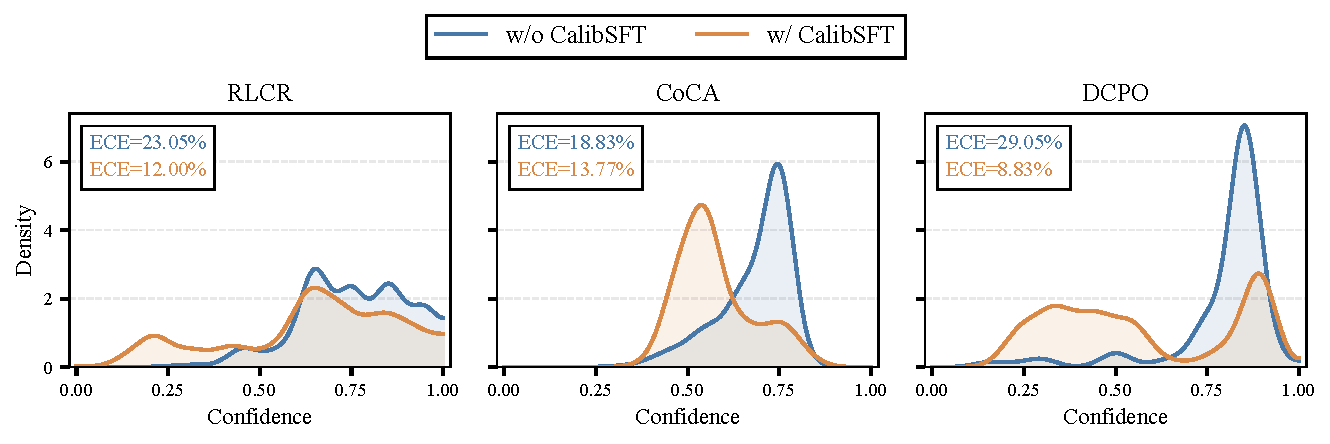
\includegraphics[width=\linewidth]{figures/minervamath_confidence_distribution.pdf}
    \caption{Confidence distributions on MinervaMath for RLCR, CoCA, and DCPO,
    with four rollouts per question at temperature 0.6.
    CalibSFT reduces concentration at dominant confidence values and lowers
    ECE for all three methods.}
    \label{fig:confidence_distribution}
\end{figure}

\paragraph{CalibSFT mitigates confidence concentration after downstream RL.}
Prior work shows that confidence estimates can remain concentrated
on a few values even after calibration-aware RL
training~\citep{wang2026process,yang2026scaling}.
To examine how CalibSFT initialization influences confidence distribution,
we compare RLCR, CoCA, and DCPO on MinervaMath.
As shown in Figure~\ref{fig:confidence_distribution}, models trained
without CalibSFT tend to concentrate their confidence on a few values and
show higher average confidence than their accuracy.
CalibSFT reduces the dominant peaks and brings average confidence closer
to accuracy, alleviating both concentration and overconfidence.
For example, DCPO's average confidence decreases from 79.32\% to 63.69\%,
while accuracy increases from 34.93\% to 36.58\%.
ECE decreases for all three methods, from 44.59\% to 28.35\% for DCPO.
We provide additional confidence distribution metrics in
Appendix~\ref{sec:confidence_distributions}.

\begin{figure}[t]
    \begin{minipage}[t]{0.55\textwidth}
        \vspace{0pt}
        \centering
        \begin{minipage}[c][3.8cm][c]{\linewidth}
            \centering
            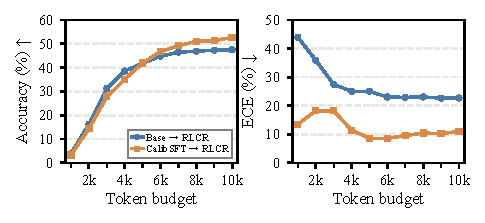
\includegraphics[width=\linewidth]{figures/aime2026_accuracy_ece.pdf}
        \end{minipage}\par
        \caption{Accuracy (left) and ECE (right) on AIME'26 across token budgets
        for RLCR with and without CalibSFT initialization. CalibSFT yields
        substantially lower ECE across all budgets while matching accuracy at
        medium budgets and improving it at larger budgets.}
        \label{fig:reasoning_budget}
    \end{minipage}\hfill
    \begin{minipage}[t]{0.42\textwidth}
        \vspace{0pt}
        \centering
        \begin{minipage}[c][3.8cm][c]{\linewidth}
        \centering
        \footnotesize
        \setlength{\tabcolsep}{3pt}
        \resizebox{\linewidth}{!}{%
\begin{tabular}{lcccc}
        \toprule
        & \multicolumn{2}{c}{Pre-SFT targets} & \multicolumn{2}{c}{Post-SFT predictions} \\
        \cmidrule(lr){2-3} \cmidrule(lr){4-5}
        Target & AUROC $\uparrow$ & Brier $\downarrow$
        & AUROC $\uparrow$ & Brier $\downarrow$ \\
        \midrule
        CSFT & 50.00 & 31.67 & 73.46 & 19.15 \\
        UaIT & 52.05 & 33.17 & 74.72 & 24.24 \\
        SaySelf & -- & 41.33 & 57.69 & 39.38 \\
        LoVeC & 75.40 & 24.71 & 71.11 & 32.32 \\
        \rowcolor{calibrow} CalibSFT & \textbf{100.00} & \textbf{7.92}
        & \textbf{79.75} & \textbf{17.81} \\
        \bottomrule
    \end{tabular}
        }
        \end{minipage}\par
        \captionof{table}{The calibration comparison between pre-SFT constructed targets and post-SFT
    predictions. CalibSFT achieves higher
    AUROC and lower Brier score across ID mathematical benchmarks.}
        \label{tab:target_construction}
    \end{minipage}
\end{figure}

\paragraph{The calibration gains of CalibSFT persist across reasoning budgets.}
To assess whether CalibSFT improves calibration as reasoning progresses
rather than the final answer alone,
we compare RLCR with and without CalibSFT initialization on AIME 2026
under varying token budgets.
As shown in Figure~\ref{fig:reasoning_budget}, CalibSFT yields substantially
lower ECE across all token budgets. It matches the RLCR baseline in accuracy
around 5,000 tokens and becomes more accurate at larger budgets.
For example, CalibSFT reduces ECE from 22.71 to 10.97 at a 10,000-token budget,
while accuracy increases from 47.50\% to 52.71\%.
These results suggest that CalibSFT's calibration benefits persist as
more computation is allocated to reasoning.

\subsection{Ablation Studies}
\label{sec:ablation_studies}



\paragraph{Confidence target construction.}

The construction of confidence targets in CalibSFT is inspired by proper scoring rules, which serve as a foundation in calibration.
To verify the effectiveness of this target design, we compare CalibSFT
with targets based on group-level correctness (CSFT)~\citep{jang2025verbalized},
token probabilities (UaIT)~\citep{liu2024uncertainty}, semantic consistency
(SaySelf)~\citep{xu2024sayself}, and rubric-based LLM judgments
(LoVeC)~\citep{zhang2026lovec}, using a shared SFT training set the same optimization objective.
We provide details of the subset and target construction in
Appendix~\ref{sec:target_construction_setup}.
We report the results of the target construction in
Table~\ref{tab:target_construction}, which shows the AUROC and Brier score of the
constructed targets before SFT and average performance on ID mathematical benchmarks after SFT. 
CalibSFT yields lower Brier score and higher
AUROC than the four alternatives. These results support the effectiveness of our confidence target
construction, which accounts for both calibration and discrimination.

\paragraph{Target mixing weight.}
\begin{wraptable}{r}{0.43\textwidth}
    \centering
    \vspace{-13pt}
    \caption{Average calibration performance on ID benchmarks across mixing
    weights. Equal weighting ($\lambda=0.5$) performs best on all three metrics.}
    \label{tab:lambda_ablation}
    \footnotesize
    \setlength{\tabcolsep}{4pt}
    \begin{tabular}{crrr}
        \toprule
        $\lambda$ & AUROC $\uparrow$ & Brier $\downarrow$ & ECE $\downarrow$ \\
        \midrule
        0 & 68.10 & 32.49 & 32.49 \\
        0.25 & 79.02 & 18.83 & 14.21 \\
        \rowcolor{calibrow} 0.5 & \textbf{79.75} & \textbf{17.81} & \textbf{13.03} \\
        0.75 & 65.93 & 19.99 & 13.16 \\
        1 & 73.29 & 19.90 & 15.04 \\
        \bottomrule
    \end{tabular}
\end{wraptable}
We construct confidence targets as
$c^*_{g,i}=\lambda q_g+(1-\lambda)z_{g,i}$, where $q_g$ is the group
success rate and $z_{g,i}$ is the correctness of an individual response.
To evaluate the effect of the mixing weight, we compare
$\lambda\in\{0,0.25,0.5,0.75,1\}$ using the same subset as above
and keeping the SFT settings fixed.
At $\lambda=0$, targets are restricted to 0 and 1; this setting yields
the highest Brier score and ECE in Table~\ref{tab:lambda_ablation}.
At $\lambda=1$, correct and incorrect responses to the same question
receive identical targets, providing no within-question discrimination
signal; post-SFT AUROC is also lower than at $\lambda=0.5$.
Equal weighting achieves the highest AUROC and lowest Brier score and ECE
among the tested settings, so we use $\lambda=0.5$ as the default.

\begin{table}[t]
    \centering
    \caption{Supervision settings and average performance on eight ID
    benchmarks. A check mark indicates that a segment contributes to the
    training loss; segment balancing averages the reasoning/answer and
    confidence losses separately. All variants use the same statically
    balanced training set and train for 180 steps.}
    \label{tab:supervision_ablation}
    \footnotesize
    \setlength{\tabcolsep}{3pt}
    \resizebox{\linewidth}{!}{%
    \begin{tabular}{lccccc rrrr}
        \toprule
        & \multicolumn{2}{c}{Reasoning/answer}
        & \multicolumn{2}{c}{Confidence}
        & Segment & \multicolumn{4}{c}{ID performance} \\
        \cmidrule(lr){2-3} \cmidrule(lr){4-5} \cmidrule(lr){7-10}
        Variant & Correct & Incorrect & Correct & Incorrect & balanced
        & Pass@1 $\uparrow$ & AUROC $\uparrow$ & Brier $\downarrow$ & ECE $\downarrow$ \\
        \midrule
        Confidence-only & -- & -- & $\checkmark$ & $\checkmark$ & --
        & 43.56 & 74.62 & 20.97 & 17.43 \\
        Full-CE & $\checkmark$ & $\checkmark$ & $\checkmark$ & $\checkmark$ & --
        & 65.89 & 61.66 & 29.29 & 27.65 \\
        Full-Balanced & $\checkmark$ & $\checkmark$ & $\checkmark$ & $\checkmark$ & $\checkmark$
        & 65.46 & 80.67 & 17.04 & \textbf{13.87} \\
        Correct-only & $\checkmark$ & -- & $\checkmark$ & -- & $\checkmark$
        & \textbf{66.59} & \textbf{81.58} & \textbf{16.95} & 14.28 \\
        \rowcolor{calibrow} CalibSFT & $\checkmark$ & -- & $\checkmark$ & $\checkmark$ & $\checkmark$
        & 65.79 & 79.30 & 17.89 & 14.36 \\
        \bottomrule
    \end{tabular}%
    }
\end{table}

\paragraph{Supervision design.}
\textbf{[TODO:]} Compare confidence-only SFT, full-completion CE,
segment-balanced full-completion CE, CalibSFT, and CalibSFT without
target-balanced sampling. Hold the training examples, confidence targets, and
optimization settings fixed across the supervision variants. Report which
completion segments contribute to each objective, followed by their ID/OOD
Pass@1 and calibration results. Use this ablation to isolate the effects of
retaining answer supervision on correct rollouts, masking incorrect reasoning
and answers, supervising confidence on all rollouts, and balancing confidence
targets.

\section{Discussion}

\subsection{Verbalized Confidence and Alternative Confidence Signals}

\paragraph{Verbalized confidence provides a directly interpretable uncertainty signal.}
\textbf{[TODO:]} Compare post-answer verbalized confidence with token- or
sequence-level probability, self-consistency, semantic consistency, and a
hidden-state probe. Use the same generated answers whenever the signal permits,
and report AUROC, Brier score, ECE, inference cost, and model-access
requirements. Discuss which gains arise from CalibSFT and which arise from the
choice of confidence signal.

\subsection{Confidence Formats and Resolution}

\paragraph{CalibSFT can be instantiated with different confidence formats.}
\textbf{[TODO:]} Compare two-decimal probabilities, discrete confidence levels,
and semantic labels such as \emph{low}, \emph{medium}, and \emph{high}. Map all
formats to $[0,1]$ for evaluation and report Pass@1, AUROC, Brier score, and
ECE. Include ConfTuner as the representative tokenized-confidence method when
its output format and evaluation mapping are matched.

\paragraph{The rollout count controls the resolution of empirical targets.}
\textbf{[TODO:]} Fix $\lambda=0.5$ and compare target construction with
$K_{\mathrm{SFT}}\in\{10,20,100\}$. Report the resulting target coverage,
target estimation cost, and final calibration. Use this comparison to separate
the effect of a finer confidence grid from the effect of additional rollout
samples.

\section{Downstream Applications}

\subsection{Selective Answering and Risk Control}

\textbf{[TODO:]} Rank responses by confidence and report risk--coverage curves,
AURC, and accuracy at matched coverage. Compare Base, confidence-aware RL, and
CalibSFT-initialized RL to test whether the calibration improvements translate
into more reliable abstention decisions.

\subsection{Confidence-Guided Efficient Reasoning}

\textbf{[TODO:]} Use confidence to allocate additional generation budget or
route uncertain questions to a stronger inference procedure. Compare against
fixed-budget and random-routing baselines at matched token cost, reporting
accuracy, calibration, and total generated tokens.

\section{Conclusion}

\textbf{[TODO:]} Summarize the concentrated and misaligned confidence prior,
the rollout-derived and target-balanced CalibSFT initialization, and its effect
on downstream confidence-aware RL. Close with the main ID/OOD evidence and the
remaining limitations of rollout-derived confidence targets.












\subsection*{AI use statement}

(This section is \textbf{required} and does not count toward the page limit.)

In this work, we used generative AI tools for [tasks with required disclosure].
We have not used generative AI tools for [other tasks with required disclosure],
and [the rest of the required disclosure tasks] are not applicable to this work.
Additionally, we used generative AI tools for [tasks with recommended¸¸
disclosure]. We have reviewed all AI-assisted work. [Elaborate. For example, “we
checked LLM-generated research ideas for potential plagiarism through a manual
literature survey”, “LLM-generated code was verified and tested for correctness
by 2 authors”, etc.]. We take responsibility for the final content of this work,
including text, claims or artifacts produced with the aid of generative AI.

See the ICLR 2027 AI Policy for Authors for more details. This statement should
not be more than 1 page.

\subsection*{Ethics statement}

(This section is \textbf{recommended} and does not count toward the page limit.)

If authors feel that their paper submission raises questions regarding the Code
of Ethics, they are encouraged to include a paragraph of Ethics Statement (at
the end of the main text before references) to address potential concerns where
appropriate. Topics include, but are not limited to, studies that involve human
subjects, practices to data set releases, potentially harmful insights,
methodologies and applications, potential conflicts of interest and sponsorship,
discrimination/bias/fairness concerns, privacy and security issues, legal
compliance, and research integrity issues (e.g., IRB, documentation, research
ethics). This statement should not be more than 1 page.

\subsection*{Reproducibility statement}

(This section is \textbf{recommended} and does not count toward the page limit.)

It is important that the work published in ICLR is reproducible. Authors are
strongly encouraged to include a paragraph-long Reproducibility Statement at the
end of the main text (before references) to discuss the efforts that have been
made to ensure reproducibility. This paragraph should not itself describe
details needed for reproducing the results, but rather reference the parts of
the main paper, appendix, and supplemental materials that will help with
reproducibility. For example, for novel models or algorithms, a link to an
anonymous downloadable source code can be submitted as supplementary materials;
for theoretical results, clear explanations of any assumptions and a complete
proof of the claims can be included in the appendix; for any datasets used in
the experiments, a complete description of the data processing steps can be
provided in the supplementary materials. Each of the above are examples of
things that can be referenced in the reproducibility statement.

\subsubsection*{Author Contributions}
If you'd like to, you may include a section for author contributions as is done
in many journals. This is optional and at the discretion of the authors.

\subsubsection*{Acknowledgments}
Use unnumbered third level headings for the acknowledgments. All
acknowledgments, including those to funding agencies, go at the end of the paper.


\bibliography{reference}
\bibliographystyle{iclr2027_conference}

\appendix

\section{Related Work}

\subsection{Confidence Estimation in LLMs}
LLM confidence can be estimated from token probabilities, hidden-state probes,
agreement across sampled answers, or explicit self-reports~\citep{kadavath2022language,
azaria2023internal,kuhn2023semantic,xiong2024can}. Verbalized-confidence methods
ask the model to emit a numerical or linguistic confidence score, providing a
single-generation estimate without requiring access to internal model
representations~\citep{tian2023just,xiong2024can}. Our work studies this
post-answer verbalized setting.

\subsection{Confidence-Aware Post-Training}
Supervised approaches train confidence outputs using correctness labels,
empirical rollout frequencies, or confidence-token objectives~\citep{lin2022teaching,
xu2024sayself,li2025conftuner}. Calibration-aware RL instead incorporates proper
scoring rewards or modifies the confidence target and credit assignment.
Representative methods include RLCR, Rewarding Doubt, CoCA, DCPO, and
CALIBER~\citep{damani2026beyond,bani2026rewarding,li2026confidence,
ma2026decoupling,finlay2026caliber}. CalibSFT focuses on the supervised
initialization supplied to these downstream RL objectives.

\section{Additional Analysis of the Motivation}
\label{sec:additional_motivation}

\subsection{Complete Confidence Distributions}
For the initial confidence analysis in Section~\ref{sec:motivation}, each
model generates ten responses to each of the same 36,915 DeepScaleR-Train
questions, with temperature 1.0, top-$p$ 0.95, and an 8,192-token budget.
We analyze the original confidence outputs before target construction.
Valid-confidence rates are 80.57\%, 99.81\%, and 79.49\% for
Qwen3-8B, Gemma4-E2B-Instruct, and OLMo3-7B-Instruct, respectively.
Distribution statistics and correctness-conditional confidence means use
valid outputs. Figure~\ref{fig:initial_confidence_prior} uses Gaussian
smoothing with bandwidth 0.04 and reflection at zero and one;
Confidence values are rounded to two decimal places before smoothing;
frequency statistics use the rounded, unsmoothed values.

\subsection{Confidence Sampling During RL}
\label{sec:motivation_training_statistics}
Table~\ref{tab:motivation_training_statistics} reports Base$\rightarrow$RLCR
statistics averaged over training steps. Confidence token entropy is the
mean next-token entropy at confidence-value token positions. Top-3 share
is the fraction of a step's sampled confidence values assigned to its
three most frequent values. Distinct confidence counts are computed
within each question's group of eight responses and then averaged.
Statistics use the groups retained by the training filter; the sampled
questions and responses can change during training.
The logged confidence values include zero placeholders for missing outputs.
Excluding all zero values, the final 40 steps still have a mean top-3 share
of 45.16\%.

\begin{table}[htbp]
    \centering
    \caption{Brier loss and confidence sampling during Base$\rightarrow$RLCR
    training. Later training lowers Brier loss while sampled confidence
    values remain concentrated.}
    \label{tab:motivation_training_statistics}
    \small
    \begin{tabular}{crrrr}
        \toprule
        Steps & Brier & Confidence token entropy & Top-3 share (\%) & Distinct values per group \\
        \midrule
        1--10 & 0.266 & 0.325 & 81.00 & 2.95 \\
        11--40 & 0.293 & 0.244 & 76.51 & 3.26 \\
        41--80 & 0.310 & 0.196 & 74.15 & 3.26 \\
        81--120 & 0.230 & 0.322 & 46.07 & 4.58 \\
        121--160 & 0.225 & 0.308 & 44.04 & 4.59 \\
        \bottomrule
    \end{tabular}
\end{table}

\subsection{Proof of Proposition~\ref{prop:confidence_saturation}}
\label{sec:confidence_saturation_proof}
\begin{proof}
We fix $h$ and the expected rewards $r_i$, and differentiate with respect
to the confidence logits.
The softmax derivative is
$\partial\pi_j/\partial\ell_i=\pi_j(\mathbf 1\{j=i\}-\pi_i)$.
It follows that
\begin{align}
    \frac{\partial J_h}{\partial\ell_i}
    &=\sum_j r_j\pi_j(\mathbf 1\{j=i\}-\pi_i) \\
    &=\pi_i(r_i-J_h).
\end{align}
Since $J_h$ is a convex combination of the $r_i$ values,
$|r_i-J_h|\leq\Delta_h$, which gives the coordinate-wise bound.
If $\pi_k=1-\varepsilon$, then
\begin{equation}
    |r_k-J_h|
    =\left|\sum_{i\ne k}\pi_i(r_k-r_i)\right|
    \leq\varepsilon\Delta_h.
\end{equation}
Consequently,
\begin{align}
    \|\nabla_\ell J_h\|_1
    &=\pi_k|r_k-J_h|+\sum_{i\ne k}\pi_i|r_i-J_h| \\
    &\leq(1-\varepsilon)\varepsilon\Delta_h
      +\varepsilon\Delta_h \\
    &\leq 2\varepsilon\Delta_h.
\end{align}
\end{proof}
The gradient is the expectation of the likelihood-ratio estimator
$R\nabla_\ell\log\pi_I$, where $I\sim\pi$ and
$R=-(c_I-Z)^2$, with $Z$ drawn from its fixed conditional distribution
given $h$, independently of $I$.
A baseline depending only on $h$ leaves this expectation unchanged.

\subsection{Proof of Proposition~\ref{prop:confidence_support}}
\label{sec:confidence_support_proof}
\begin{proof}
Conditional independence gives
$\mathbb E[Z-p_h\mid h,C]=0$. Expanding the square therefore yields
\begin{align}
    \mathbb E[(C-Z)^2\mid h]
    &=\mathbb E[(Z-p_h)^2\mid h]
      +\mathbb E[(C-p_h)^2\mid h] \\
    &=p_h(1-p_h)+\mathbb E[(C-p_h)^2\mid h].
\end{align}
For any $\delta>0$, the second term satisfies
\begin{align}
    \mathbb E[(C-Z)^2\mid h]-p_h(1-p_h)
    &=\mathbb E[(C-p_h)^2\mid h] \\
    &\geq\delta^2\Pr(|C-p_h|\geq\delta\mid h) \\
    &=\delta^2(1-m_\delta(h)).
\end{align}
Thus, assigning little probability mass near $p_h$ incurs excess Brier
loss even when confidence values in that neighborhood remain possible.
\end{proof}

\paragraph{Restricted confidence support.}
As a special case, suppose $\Pr(C\in S_h\mid h)=1$ for a nonempty
set $S_h\subseteq[0,1]$, and define
$d_h=\operatorname{dist}(p_h,S_h)=\inf_{c\in S_h}|c-p_h|$.
If $d_h>0$, then $m_{d_h}(h)=0$, and
Proposition~\ref{prop:confidence_support} with $\delta=d_h$ gives
\begin{equation}
    \mathbb E[(C-Z)^2\mid h]
    \geq p_h(1-p_h)+\operatorname{dist}(p_h,S_h)^2.
\end{equation}
For $d_h=0$, the same bound follows directly from the decomposition above.
If $S_h$ is closed, a predictor that always outputs a nearest point in
$S_h$ attains the bound.

\paragraph{Finite-sampling limitation.}
Fix the policy and prediction information $h$, and draw $G$ independent
confidence samples $C_1,\ldots,C_G$ from its conditional distribution.
Each confidence sample lies outside
$\{c:|c-p_h|<\delta\}$ with probability $1-m_\delta(h)$.
Independence gives the probability $(1-m_\delta(h))^G$ that all $G$
samples lie outside. On that event, even the sample closest to $p_h$
has squared error at least $\delta^2$, so
\begin{equation}
    \mathbb E\!\left[\min_{i\leq G}(C_i-p_h)^2\mid h\right]
    \geq\delta^2(1-m_\delta(h))^G.
\end{equation}
Here $p_h$ is conditional on the information used for a particular
prediction, rather than the prompt's average success rate across different
answers. The sampling statement fixes this information and the policy;
it does not assume that support remains unchanged during RL.

\subsection{Additional Models and Sampling Settings}
\textbf{[TODO:]} Add the motivation analysis for additional model families and
sampling settings once those evaluation runs are complete.

\section{Implementation Details}
\label{sec:detailed_setup}

\subsection{Training Pipelines}

All runs use Qwen3-8B as the base model. We randomly hold out 2,000 examples
from DeepScaleR-Preview as a test split (DeepScaleR-Eval) and use all remaining
examples as the training split (DeepScaleR-Train), which is used to
construct the SFT data for CalibSFT and the downstream RL training data.

\paragraph{CalibSFT.}
To construct CalibSFT targets, we sample 10 rollouts per prompt from
DeepScaleR-Train with temperature 1.0 and top-$p$ 0.95. We compute 
its group success rate, and combine group-level and rollout-level
correctness with $\lambda=0.5$. We use target-balanced sampling and the
selective completion mask with $\beta=0.5$: correct rollouts supervise both the
reasoning/answer and confidence segments, whereas incorrect rollouts supervise
only the confidence segment. Generally, we train CalibSFT for 180 steps with a
learning rate of $2\times10^{-6}$ and 10 warm-up steps.

\paragraph{Confidence-aware RL.}
For downstream RL, each prompt group contains 8 sampled responses, with each
response capped at 8,192 tokens. We train with batches of 64 prompt groups for
160 optimization steps. For methods using DAPO dynamic sampling, this
corresponds to approximately 600 rollout-generation batches. Dynamic sampling retains only groups
with mixed correctness outcomes and discards groups whose responses are all
correct or all incorrect. To accelerate training for these methods, we
remove questions for which all sampled responses from the base model are
correct before RL training begins. Each method retains its own reward and
credit assignment.

\begin{itemize}
    \item \textbf{Direct RL baselines.} RLVR, RLCR~\citep{damani2026beyond}, CoCA~\citep{li2026confidence}, and DCPO~\citep{ma2026decoupling} are trained
    directly from the Qwen3-8B base checkpoint. They share the DAPO training
    recipe but retain their respective correctness, calibration-target, and
    credit-assignment objectives.
    \item \textbf{ReDoubt.} ReDoubt is initialized from the
    trained RLVR checkpoint and then optimized with its clipped log-score
    confidence objective~\citep{bani2026rewarding}. When incorporated with CalibSFT, we first train CalibSFT on the RLVR checkpoint and then continue with ReDoubt RL.
    \item \textbf{C3RL.} C3RL~\citep{yang2026scaling} combines correctness,
    calibration, and reference-accuracy rewards. C3RL uses the
    digit confidence format, expressing confidence as an integer from 0 to 9
    and mapping it to $[0,1]$ by dividing by 9. The CalibSFT initialization
    for C3RL is also trained in this format. We use the base model's
    rollout success rates to label each training question as all correct,
    partially correct, or all incorrect. The reference reward encourages
    correct answers to previously all-incorrect questions and penalizes
    incorrect answers to previously all-correct questions. To retain these
    questions and their reference-reward signals, we disable DAPO dynamic
    sampling and all-correct filtering, using the full RL training split
    for C3RL both with and without CalibSFT initialization.
\end{itemize}

\subsection{Evaluation Protocol}
For the main results, we use temperature $0.6$ and sample four rollouts per
question on non-AIME mathematical and OOD benchmarks and 32 rollouts per
question on AIME. Pass@1 is the mean correctness over these sampled rollouts.
The supervision and target ablations retain their recorded evaluation settings.
Confidence is parsed from the final probability field and normalized to $[0,1]$.
We use 10 equal-width bins for calculating ECE. Unless otherwise noted, RL results use
the final checkpoint after 160 optimization steps, while SFT-only results use
the checkpoint at the end of their respective SFT runs.

\section{Detailed Experimental Results}

\subsection{Per-Dataset Main Results}
\label{sec:per_dataset_results}
Table~\ref{tab:main_results} reports split-level averages. The following tables
expose the same metrics for every benchmark; the final cell in each split is
the unweighted average over its datasets.

\newcommand{\appendixdatasettable}[2]{%
\begin{subtable}[t]{0.32\textwidth}
\centering
\caption{#1}
\scriptsize
\setlength{\tabcolsep}{2pt}
\renewcommand\arraystretch{0.92}
\begin{tabular}{lcccc}
\toprule
Method & P@1 & AUROC & Brier & ECE \\
\midrule
#2
\bottomrule
\end{tabular}
\end{subtable}%
}

\begin{table*}[p]
\centering
\caption{Per-dataset results on the in-domain mathematical benchmarks. Base,
RLVR, and standalone CalibSFT use 6,144 tokens; downstream RL models use
16,384 tokens. Temperature is 0.6, with four rollouts per non-AIME question
and 32 per AIME question.}
\label{tab:appendix_id_results}
\appendixdatasettable{DeepScaleR-Eval}{
Base & 60.84 & 66.31 & 34.09 & 34.06 \\
RLVR & \textbf{70.15} & 68.11 & 26.94 & 26.37 \\
\rowcolor{calibrow} CalibSFT & 60.88 & \textbf{73.76} & \textbf{23.60} & \textbf{17.57} \\
\midrule
RLCR & 71.24 & 75.33 & 16.65 & 5.14 \\
\rowcolor{calibrow} + CalibSFT & \textbf{72.47} & \textbf{79.34} & \textbf{15.33} & \textbf{4.58} \\
\midrule
ReDoubt & 71.53 & 75.92 & 17.13 & 10.28 \\
\rowcolor{calibrow} + CalibSFT & \textbf{71.92} & \textbf{79.91} & \textbf{15.08} & \textbf{3.65} \\
\midrule
CoCA & 70.16 & 73.17 & 17.73 & 8.51 \\
\rowcolor{calibrow} + CalibSFT & \textbf{71.45} & \textbf{78.71} & \textbf{16.41} & \textbf{7.92} \\
\midrule
DCPO & \textbf{71.45} & 71.74 & 17.30 & 6.50 \\
\rowcolor{calibrow} + CalibSFT & 70.46 & \textbf{77.71} & \textbf{16.06} & \textbf{5.95} \\
\midrule
C3RL & 70.65 & 62.87 & 24.64 & 25.05 \\
\rowcolor{calibrow} + CalibSFT & \textbf{71.05} & \textbf{71.91} & \textbf{19.93} & \textbf{14.72} \\
}\hfill
\appendixdatasettable{MATH-500}{
Base & 83.90 & 63.80 & 14.78 & 13.87 \\
RLVR & \textbf{89.15} & 67.69 & \textbf{10.13} & \textbf{8.76} \\
\rowcolor{calibrow} CalibSFT & 83.65 & \textbf{82.11} & 14.70 & 11.53 \\
\midrule
RLCR & \textbf{90.50} & 76.39 & 7.54 & 7.43 \\
\rowcolor{calibrow} + CalibSFT & 90.15 & \textbf{89.79} & \textbf{6.56} & \textbf{3.69} \\
\midrule
ReDoubt & \textbf{90.05} & 74.85 & 9.82 & 15.01 \\
\rowcolor{calibrow} + CalibSFT & 89.45 & \textbf{88.92} & \textbf{7.87} & \textbf{10.41} \\
\midrule
CoCA & \textbf{89.85} & 72.69 & 10.64 & 18.18 \\
\rowcolor{calibrow} + CalibSFT & \textbf{89.85} & \textbf{87.29} & \textbf{9.09} & \textbf{15.49} \\
\midrule
DCPO & 89.30 & 70.77 & 7.90 & \textbf{6.27} \\
\rowcolor{calibrow} + CalibSFT & \textbf{90.20} & \textbf{84.89} & \textbf{7.68} & 7.70 \\
\midrule
C3RL & \textbf{89.40} & 60.22 & \textbf{9.42} & 9.75 \\
\rowcolor{calibrow} + CalibSFT & 87.70 & \textbf{84.76} & 10.37 & \textbf{9.36} \\
}\hfill
\appendixdatasettable{MinervaMath}{
Base & \textbf{39.89} & \textbf{63.26} & 53.79 & 55.28 \\
RLVR & 37.96 & 60.92 & 57.18 & 58.40 \\
\rowcolor{calibrow} CalibSFT & \textbf{39.89} & 57.50 & \textbf{30.33} & \textbf{24.20} \\
\midrule
RLCR & 36.67 & 66.67 & 35.91 & 38.12 \\
\rowcolor{calibrow} + CalibSFT & \textbf{37.04} & \textbf{76.29} & \textbf{26.81} & \textbf{26.33} \\
\midrule
ReDoubt & \textbf{37.59} & 66.65 & 27.92 & 25.37 \\
\rowcolor{calibrow} + CalibSFT & 37.50 & \textbf{81.81} & \textbf{18.41} & \textbf{16.15} \\
\midrule
CoCA & 35.20 & 65.28 & 32.43 & 33.26 \\
\rowcolor{calibrow} + CalibSFT & \textbf{36.95} & \textbf{78.62} & \textbf{23.47} & \textbf{24.42} \\
\midrule
DCPO & 34.93 & 64.19 & 41.78 & 44.59 \\
\rowcolor{calibrow} + CalibSFT & \textbf{36.86} & \textbf{74.73} & \textbf{23.33} & \textbf{20.25} \\
\midrule
C3RL & \textbf{37.22} & 56.00 & 58.42 & 59.49 \\
\rowcolor{calibrow} + CalibSFT & 35.85 & \textbf{77.64} & \textbf{20.14} & \textbf{16.95} \\
}

\medskip
\appendixdatasettable{OlympiadBench}{
Base & 54.41 & 69.82 & 38.93 & 40.13 \\
RLVR & \textbf{56.31} & 72.84 & 39.35 & 39.98 \\
\rowcolor{calibrow} CalibSFT & 51.67 & \textbf{79.33} & \textbf{22.48} & \textbf{20.62} \\
\midrule
RLCR & 57.83 & 81.78 & 19.04 & \textbf{12.50} \\
\rowcolor{calibrow} + CalibSFT & \textbf{58.46} & \textbf{89.71} & \textbf{16.09} & 13.25 \\
\midrule
ReDoubt & 57.57 & 80.67 & 18.18 & \textbf{8.36} \\
\rowcolor{calibrow} + CalibSFT & \textbf{59.90} & \textbf{91.00} & \textbf{12.67} & 9.38 \\
\midrule
CoCA & \textbf{56.38} & 80.19 & 20.14 & \textbf{14.63} \\
\rowcolor{calibrow} + CalibSFT & 56.19 & \textbf{90.47} & \textbf{18.09} & 20.16 \\
\midrule
DCPO & 57.05 & 78.43 & 21.85 & 17.75 \\
\rowcolor{calibrow} + CalibSFT & \textbf{57.46} & \textbf{88.53} & \textbf{15.72} & \textbf{12.14} \\
\midrule
C3RL & \textbf{57.68} & 62.66 & 35.85 & 37.52 \\
\rowcolor{calibrow} + CalibSFT & 56.64 & \textbf{84.53} & \textbf{17.91} & \textbf{18.60} \\
}\hfill
\appendixdatasettable{GSM8K}{
Base & 94.35 & 67.82 & 5.20 & 3.39 \\
RLVR & \textbf{94.64} & 67.97 & \textbf{5.06} & \textbf{3.05} \\
\rowcolor{calibrow} CalibSFT & 94.31 & \textbf{70.24} & 17.90 & 20.78 \\
\midrule
RLCR & \textbf{94.81} & 78.88 & 4.77 & 5.58 \\
\rowcolor{calibrow} + CalibSFT & 94.67 & \textbf{82.60} & \textbf{4.64} & \textbf{2.72} \\
\midrule
ReDoubt & \textbf{94.96} & \textbf{78.40} & 7.07 & 16.27 \\
\rowcolor{calibrow} + CalibSFT & 94.86 & 77.91 & \textbf{5.76} & \textbf{10.92} \\
\midrule
CoCA & \textbf{94.58} & 69.00 & 8.94 & 21.02 \\
\rowcolor{calibrow} + CalibSFT & 94.56 & \textbf{71.85} & \textbf{8.26} & \textbf{18.10} \\
\midrule
DCPO & \textbf{94.48} & 68.34 & \textbf{5.50} & 9.13 \\
\rowcolor{calibrow} + CalibSFT & 94.45 & \textbf{73.40} & 5.80 & \textbf{7.48} \\
\midrule
C3RL & \textbf{94.37} & 57.25 & 5.33 & 5.24 \\
\rowcolor{calibrow} + CalibSFT & 94.29 & \textbf{64.91} & \textbf{5.26} & \textbf{5.08} \\
}\hfill
\appendixdatasettable{AIME2024}{
Base & 48.23 & 81.93 & 39.61 & 42.50 \\
RLVR & \textbf{52.92} & 82.05 & 39.49 & 41.15 \\
\rowcolor{calibrow} CalibSFT & 45.42 & \textbf{89.96} & \textbf{11.93} & \textbf{6.03} \\
\midrule
RLCR & 59.48 & \textbf{93.59} & 13.17 & 19.70 \\
\rowcolor{calibrow} + CalibSFT & \textbf{64.17} & 92.42 & \textbf{10.97} & \textbf{9.79} \\
\midrule
ReDoubt & 55.62 & 91.94 & 15.40 & 22.77 \\
\rowcolor{calibrow} + CalibSFT & \textbf{63.23} & \textbf{92.72} & \textbf{10.04} & \textbf{10.34} \\
\midrule
CoCA & 53.85 & 92.22 & \textbf{16.27} & \textbf{21.37} \\
\rowcolor{calibrow} + CalibSFT & \textbf{58.54} & \textbf{95.41} & 16.34 & 23.56 \\
\midrule
DCPO & 57.92 & 88.84 & 12.32 & \textbf{8.47} \\
\rowcolor{calibrow} + CalibSFT & \textbf{58.33} & \textbf{93.89} & \textbf{11.02} & 11.85 \\
\midrule
C3RL & 59.69 & 80.93 & 25.25 & 30.19 \\
\rowcolor{calibrow} + CalibSFT & \textbf{64.27} & \textbf{85.24} & \textbf{14.04} & \textbf{12.99} \\
}

\medskip
\appendixdatasettable{AIME2025}{
Base & 35.00 & 82.75 & 48.25 & 52.81 \\
RLVR & \textbf{43.44} & 84.95 & 45.87 & 49.00 \\
\rowcolor{calibrow} CalibSFT & 34.27 & \textbf{92.48} & \textbf{9.95} & \textbf{8.02} \\
\midrule
RLCR & 43.33 & \textbf{95.53} & \textbf{13.60} & 23.06 \\
\rowcolor{calibrow} + CalibSFT & \textbf{48.02} & 92.40 & 13.87 & \textbf{14.28} \\
\midrule
ReDoubt & 44.90 & 94.22 & 15.19 & 26.51 \\
\rowcolor{calibrow} + CalibSFT & \textbf{50.52} & \textbf{95.28} & \textbf{10.11} & \textbf{10.84} \\
\midrule
CoCA & 40.31 & \textbf{95.39} & \textbf{17.04} & 29.31 \\
\rowcolor{calibrow} + CalibSFT & \textbf{45.00} & 94.21 & 19.99 & \textbf{26.43} \\
\midrule
DCPO & 41.15 & 91.19 & \textbf{13.33} & \textbf{14.30} \\
\rowcolor{calibrow} + CalibSFT & \textbf{41.25} & \textbf{95.07} & 13.81 & 17.73 \\
\midrule
C3RL & \textbf{43.96} & 79.01 & 36.25 & 42.69 \\
\rowcolor{calibrow} + CalibSFT & 43.12 & \textbf{86.74} & \textbf{21.86} & \textbf{25.49} \\
}\hfill
\appendixdatasettable{AIME2026}{
Base & 42.50 & 76.08 & 45.13 & 48.07 \\
RLVR & \textbf{48.23} & 80.70 & 43.82 & 45.92 \\
\rowcolor{calibrow} CalibSFT & 39.48 & \textbf{88.65} & \textbf{13.22} & \textbf{9.79} \\
\midrule
RLCR & 47.81 & \textbf{94.10} & 14.08 & 23.19 \\
\rowcolor{calibrow} + CalibSFT & \textbf{52.60} & 92.48 & \textbf{13.57} & \textbf{12.04} \\
\midrule
ReDoubt & 52.40 & 90.93 & 16.78 & 26.20 \\
\rowcolor{calibrow} + CalibSFT & \textbf{53.75} & \textbf{94.57} & \textbf{9.54} & \textbf{10.42} \\
\midrule
CoCA & 48.54 & \textbf{96.74} & \textbf{14.84} & 27.72 \\
\rowcolor{calibrow} + CalibSFT & \textbf{48.65} & 93.96 & 19.52 & \textbf{25.63} \\
\midrule
DCPO & 49.58 & 91.78 & \textbf{11.04} & \textbf{10.41} \\
\rowcolor{calibrow} + CalibSFT & \textbf{50.21} & \textbf{93.07} & 12.87 & 14.52 \\
\midrule
C3RL & 52.81 & 84.29 & 27.21 & 33.72 \\
\rowcolor{calibrow} + CalibSFT & \textbf{53.65} & \textbf{91.31} & \textbf{15.69} & \textbf{18.30} \\
}\hfill
\appendixdatasettable{Overall (ID)}{
Base & 57.39 & 71.47 & 34.97 & 36.26 \\
RLVR & \textbf{61.60} & 73.16 & 33.48 & 34.08 \\
\rowcolor{calibrow} CalibSFT & 56.20 & \textbf{79.25} & \textbf{18.01} & \textbf{14.82} \\
\midrule
RLCR & 62.71 & 82.78 & 15.60 & 16.84 \\
\rowcolor{calibrow} + CalibSFT & \textbf{64.70} & \textbf{86.88} & \textbf{13.48} & \textbf{10.84} \\
\midrule
ReDoubt & 63.08 & 81.70 & 15.94 & 18.85 \\
\rowcolor{calibrow} + CalibSFT & \textbf{65.14} & \textbf{87.76} & \textbf{11.18} & \textbf{10.26} \\
\midrule
CoCA & 61.11 & 80.59 & 17.25 & 21.75 \\
\rowcolor{calibrow} + CalibSFT & \textbf{62.65} & \textbf{86.31} & \textbf{16.40} & \textbf{20.21} \\
\midrule
DCPO & 61.98 & 78.16 & 16.38 & 14.68 \\
\rowcolor{calibrow} + CalibSFT & \textbf{62.40} & \textbf{85.16} & \textbf{13.29} & \textbf{12.20} \\
\midrule
C3RL & 63.22 & 67.90 & 27.80 & 30.45 \\
\rowcolor{calibrow} + CalibSFT & \textbf{63.32} & \textbf{80.88} & \textbf{15.65} & \textbf{15.18} \\
}
\end{table*}

\begin{table*}[p]
\centering
\caption{Per-dataset results on the revised eight-dataset out-of-domain suite.
Each question has four sampled responses at temperature 0.6.
WebQuestions contains only examples with a single gold answer.}
\label{tab:appendix_ood_results}
\appendixdatasettable{HotpotQA}{
Base & 64.68 & \textbf{57.68} & 32.82 & 32.16 \\
RLVR & 64.58 & 54.16 & 33.10 & 32.17 \\
\rowcolor{calibrow} CalibSFT & \textbf{65.70} & 54.18 & \textbf{29.38} & \textbf{20.57} \\
\midrule
RLCR & 65.80 & 59.10 & 25.97 & 19.77 \\
\rowcolor{calibrow} + CalibSFT & \textbf{66.27} & \textbf{59.23} & \textbf{24.25} & \textbf{10.85} \\
\midrule
ReDoubt & 64.83 & 60.64 & 23.52 & 12.11 \\
\rowcolor{calibrow} + CalibSFT & \textbf{65.90} & \textbf{62.57} & \textbf{21.83} & \textbf{6.19} \\
\midrule
CoCA & 64.90 & 56.43 & \textbf{22.77} & \textbf{6.02} \\
\rowcolor{calibrow} + CalibSFT & \textbf{66.10} & \textbf{61.57} & 22.92 & 11.39 \\
\midrule
DCPO & \textbf{66.15} & 57.88 & 25.33 & 18.77 \\
\rowcolor{calibrow} + CalibSFT & 65.97 & \textbf{60.70} & \textbf{24.43} & \textbf{14.92} \\
\midrule
C3RL & 65.38 & 52.47 & 33.39 & 33.12 \\
\rowcolor{calibrow} + CalibSFT & \textbf{66.50} & \textbf{58.94} & \textbf{28.45} & \textbf{19.78} \\
}\hfill
\appendixdatasettable{TriviaQA}{
Base & \textbf{55.24} & 75.80 & 35.68 & 36.93 \\
RLVR & 54.97 & \textbf{76.01} & 40.59 & 41.40 \\
\rowcolor{calibrow} CalibSFT & 55.21 & 65.05 & \textbf{28.44} & \textbf{20.98} \\
\midrule
RLCR & 55.24 & \textbf{81.66} & 23.84 & 23.30 \\
\rowcolor{calibrow} + CalibSFT & \textbf{55.25} & 81.53 & \textbf{18.89} & \textbf{10.71} \\
\midrule
ReDoubt & 55.69 & 82.96 & 18.67 & 13.58 \\
\rowcolor{calibrow} + CalibSFT & \textbf{56.20} & \textbf{84.23} & \textbf{17.72} & \textbf{10.89} \\
\midrule
CoCA & 54.77 & 77.62 & 21.63 & \textbf{12.97} \\
\rowcolor{calibrow} + CalibSFT & \textbf{54.89} & \textbf{81.85} & \textbf{20.98} & 13.16 \\
\midrule
DCPO & 54.55 & 79.86 & 25.93 & 23.91 \\
\rowcolor{calibrow} + CalibSFT & \textbf{55.12} & \textbf{82.56} & \textbf{17.59} & \textbf{8.25} \\
\midrule
C3RL & 53.76 & \textbf{73.01} & 35.61 & 38.53 \\
\rowcolor{calibrow} + CalibSFT & \textbf{54.11} & 71.36 & \textbf{22.75} & \textbf{12.50} \\
}\hfill
\appendixdatasettable{DROP}{
Base & 80.36 & 59.13 & 18.22 & 17.03 \\
RLVR & \textbf{83.53} & 59.32 & \textbf{15.34} & \textbf{13.31} \\
\rowcolor{calibrow} CalibSFT & 79.92 & \textbf{59.38} & 31.60 & 28.93 \\
\midrule
RLCR & 81.44 & 63.34 & \textbf{14.72} & \textbf{5.43} \\
\rowcolor{calibrow} + CalibSFT & \textbf{82.32} & \textbf{74.44} & 14.99 & 10.75 \\
\midrule
ReDoubt & \textbf{83.63} & 63.27 & 14.76 & \textbf{10.80} \\
\rowcolor{calibrow} + CalibSFT & 81.69 & \textbf{79.08} & \textbf{14.10} & 13.24 \\
\midrule
CoCA & 82.47 & 61.58 & \textbf{15.03} & \textbf{11.56} \\
\rowcolor{calibrow} + CalibSFT & \textbf{82.50} & \textbf{73.91} & 17.95 & 21.99 \\
\midrule
DCPO & \textbf{83.45} & 59.34 & \textbf{13.25} & \textbf{2.30} \\
\rowcolor{calibrow} + CalibSFT & 80.42 & \textbf{75.92} & 16.54 & 13.64 \\
\midrule
C3RL & \textbf{82.65} & 54.56 & \textbf{16.37} & \textbf{16.07} \\
\rowcolor{calibrow} + CalibSFT & 77.44 & \textbf{64.78} & 23.65 & 22.03 \\
}

\medskip
\appendixdatasettable{MuSiQue}{
Base & 45.84 & \textbf{62.90} & 41.91 & 42.33 \\
RLVR & 47.18 & 58.12 & 46.19 & 46.75 \\
\rowcolor{calibrow} CalibSFT & \textbf{47.19} & 62.25 & \textbf{26.51} & \textbf{13.95} \\
\midrule
RLCR & 47.77 & 66.21 & 25.68 & 15.35 \\
\rowcolor{calibrow} + CalibSFT & \textbf{49.97} & \textbf{67.87} & \textbf{23.22} & \textbf{6.13} \\
\midrule
ReDoubt & 46.90 & 66.37 & 24.07 & 11.21 \\
\rowcolor{calibrow} + CalibSFT & \textbf{49.66} & \textbf{71.54} & \textbf{21.59} & \textbf{3.65} \\
\midrule
CoCA & 46.69 & \textbf{67.03} & 23.69 & 10.18 \\
\rowcolor{calibrow} + CalibSFT & \textbf{48.76} & 66.88 & \textbf{23.56} & \textbf{7.72} \\
\midrule
DCPO & 47.34 & 65.48 & 28.28 & 20.53 \\
\rowcolor{calibrow} + CalibSFT & \textbf{48.96} & \textbf{70.49} & \textbf{22.75} & \textbf{8.55} \\
\midrule
C3RL & 45.55 & 63.39 & 39.88 & 40.04 \\
\rowcolor{calibrow} + CalibSFT & \textbf{47.47} & \textbf{66.39} & \textbf{24.46} & \textbf{11.87} \\
}\hfill
\appendixdatasettable{LiveBenchReasoning}{
Base & 52.88 & 61.81 & 40.53 & 40.59 \\
RLVR & 29.25 & 60.32 & 61.75 & 64.59 \\
\rowcolor{calibrow} CalibSFT & \textbf{53.00} & \textbf{67.67} & \textbf{25.40} & \textbf{17.74} \\
\midrule
RLCR & 31.75 & 68.00 & 28.49 & 29.09 \\
\rowcolor{calibrow} + CalibSFT & \textbf{42.25} & \textbf{68.41} & \textbf{21.94} & \textbf{7.75} \\
\midrule
ReDoubt & 25.75 & 68.44 & 23.51 & 24.86 \\
\rowcolor{calibrow} + CalibSFT & \textbf{47.12} & \textbf{86.43} & \textbf{18.27} & \textbf{15.36} \\
\midrule
CoCA & 32.12 & 66.75 & 25.79 & 23.64 \\
\rowcolor{calibrow} + CalibSFT & \textbf{41.50} & \textbf{68.03} & \textbf{23.24} & \textbf{7.96} \\
\midrule
DCPO & 31.13 & 67.14 & 32.10 & 33.12 \\
\rowcolor{calibrow} + CalibSFT & \textbf{37.75} & \textbf{71.77} & \textbf{21.12} & \textbf{8.83} \\
\midrule
C3RL & 33.00 & \textbf{57.18} & 53.55 & 55.46 \\
\rowcolor{calibrow} + CalibSFT & \textbf{44.62} & 53.33 & \textbf{28.11} & \textbf{22.78} \\
}\hfill
\appendixdatasettable{NQOpen}{
Base & 21.12 & 66.31 & 66.04 & 70.59 \\
RLVR & \textbf{24.13} & \textbf{67.07} & 68.92 & 71.55 \\
\rowcolor{calibrow} CalibSFT & 21.64 & 59.59 & \textbf{27.33} & \textbf{29.16} \\
\midrule
RLCR & 23.32 & 70.48 & 43.84 & 52.43 \\
\rowcolor{calibrow} + CalibSFT & \textbf{23.80} & \textbf{72.24} & \textbf{26.44} & \textbf{30.89} \\
\midrule
ReDoubt & \textbf{24.67} & 70.28 & 32.15 & 39.19 \\
\rowcolor{calibrow} + CalibSFT & 23.81 & \textbf{73.10} & \textbf{25.69} & \textbf{31.16} \\
\midrule
CoCA & 22.76 & 66.59 & 35.28 & 43.26 \\
\rowcolor{calibrow} + CalibSFT & \textbf{23.72} & \textbf{70.77} & \textbf{24.86} & \textbf{28.69} \\
\midrule
DCPO & \textbf{23.69} & 69.80 & 46.27 & 53.69 \\
\rowcolor{calibrow} + CalibSFT & 23.58 & \textbf{73.13} & \textbf{22.65} & \textbf{25.97} \\
\midrule
C3RL & \textbf{22.43} & \textbf{64.77} & 63.63 & 68.49 \\
\rowcolor{calibrow} + CalibSFT & 22.08 & 61.18 & \textbf{22.25} & \textbf{17.54} \\
}

\medskip
\appendixdatasettable{PopQA}{
Base & 20.85 & \textbf{74.94} & 57.89 & 64.10 \\
RLVR & \textbf{21.37} & 72.78 & 68.14 & 71.96 \\
\rowcolor{calibrow} CalibSFT & 21.00 & 63.88 & \textbf{24.80} & \textbf{26.68} \\
\midrule
RLCR & \textbf{21.29} & \textbf{76.88} & 37.71 & 47.90 \\
\rowcolor{calibrow} + CalibSFT & 21.16 & 76.55 & \textbf{24.76} & \textbf{32.22} \\
\midrule
ReDoubt & \textbf{21.37} & 76.83 & 26.82 & 36.23 \\
\rowcolor{calibrow} + CalibSFT & 21.30 & \textbf{80.27} & \textbf{23.63} & \textbf{31.90} \\
\midrule
CoCA & \textbf{21.06} & 73.92 & 30.84 & 39.88 \\
\rowcolor{calibrow} + CalibSFT & 20.88 & \textbf{76.99} & \textbf{24.12} & \textbf{31.76} \\
\midrule
DCPO & 20.99 & \textbf{77.02} & 41.10 & 49.96 \\
\rowcolor{calibrow} + CalibSFT & \textbf{21.18} & 76.52 & \textbf{21.29} & \textbf{28.02} \\
\midrule
C3RL & \textbf{20.81} & \textbf{71.98} & 54.60 & 61.92 \\
\rowcolor{calibrow} + CalibSFT & 20.66 & 66.98 & \textbf{16.56} & \textbf{12.95} \\
}\hfill
\appendixdatasettable{WebQuestions}{
Base & 21.88 & \textbf{67.10} & 68.16 & 71.80 \\
RLVR & \textbf{26.02} & 65.76 & 68.29 & 70.41 \\
\rowcolor{calibrow} CalibSFT & 23.59 & 59.02 & \textbf{32.52} & \textbf{35.25} \\
\midrule
RLCR & \textbf{25.07} & 69.40 & 48.86 & 56.11 \\
\rowcolor{calibrow} + CalibSFT & 24.63 & \textbf{70.20} & \textbf{31.41} & \textbf{36.33} \\
\midrule
ReDoubt & \textbf{26.84} & 70.22 & 37.08 & 43.81 \\
\rowcolor{calibrow} + CalibSFT & 25.02 & \textbf{70.67} & \textbf{29.34} & \textbf{34.89} \\
\midrule
CoCA & 24.65 & 64.40 & 38.35 & 45.46 \\
\rowcolor{calibrow} + CalibSFT & \textbf{26.06} & \textbf{69.71} & \textbf{25.93} & \textbf{28.47} \\
\midrule
DCPO & 24.59 & 68.48 & 50.52 & 57.04 \\
\rowcolor{calibrow} + CalibSFT & \textbf{25.61} & \textbf{70.87} & \textbf{27.45} & \textbf{30.32} \\
\midrule
C3RL & \textbf{23.94} & 60.19 & 67.27 & 70.35 \\
\rowcolor{calibrow} + CalibSFT & \textbf{23.94} & \textbf{61.29} & \textbf{24.87} & \textbf{19.55} \\
}\hfill
\appendixdatasettable{Overall (OOD)}{
Base & 45.36 & \textbf{65.71} & 45.15 & 46.94 \\
RLVR & 43.88 & 64.19 & 50.29 & 51.52 \\
\rowcolor{calibrow} CalibSFT & \textbf{45.91} & 61.38 & \textbf{28.25} & \textbf{24.16} \\
\midrule
RLCR & 43.96 & 69.38 & 31.14 & 31.17 \\
\rowcolor{calibrow} + CalibSFT & \textbf{45.71} & \textbf{71.31} & \textbf{23.24} & \textbf{18.20} \\
\midrule
ReDoubt & 43.71 & 69.88 & 25.07 & 23.98 \\
\rowcolor{calibrow} + CalibSFT & \textbf{46.34} & \textbf{75.98} & \textbf{21.52} & \textbf{18.41} \\
\midrule
CoCA & 43.68 & 66.79 & 26.67 & 24.12 \\
\rowcolor{calibrow} + CalibSFT & \textbf{45.55} & \textbf{71.21} & \textbf{22.95} & \textbf{18.89} \\
\midrule
DCPO & 43.99 & 68.13 & 32.85 & 32.41 \\
\rowcolor{calibrow} + CalibSFT & \textbf{44.82} & \textbf{72.75} & \textbf{21.73} & \textbf{17.31} \\
\midrule
C3RL & 43.44 & 62.19 & 45.54 & 48.00 \\
\rowcolor{calibrow} + CalibSFT & \textbf{44.60} & \textbf{63.03} & \textbf{23.89} & \textbf{17.38} \\
}
\end{table*}


\subsection{Ablation of SFT Confidence Targets}
\label{sec:target_construction_setup}

\begin{wraptable}{r}{0.5\textwidth}
    \centering
    \vspace{-13pt}
    \caption{Training-target distribution (\%) over ten equal-width bins in the confidence target ablation.}
    \label{tab:training_target_distribution}
    \footnotesize
    \setlength{\tabcolsep}{3pt}
    \begin{tabular}{crrrrr}
        \toprule
        Interval & CSFT & UaIT & SaySelf & LoVeC & CalibSFT \\
        \midrule
        $[0.0, 0.1]$ & 11.11 & 0.00 & 22.07 & 27.33 & 11.11 \\
        $(0.1, 0.2]$ & 11.11 & 0.00 & 14.41 & 3.78 & 11.11 \\
        $(0.2, 0.3]$ & 11.11 & 0.00 & 11.93 & 8.17 & 11.11 \\
        $(0.3, 0.4]$ & 11.11 & 0.00 & 10.22 & 0.20 & 11.11 \\
        $(0.4, 0.5]$ & 11.11 & 0.00 & 9.04 & 1.37 & 5.56 \\
        $(0.5, 0.6]$ & 11.11 & 0.00 & 8.26 & 0.63 & 11.11 \\
        $(0.6, 0.7]$ & 11.11 & 6.48 & 8.89 & 0.22 & 11.11 \\
        $(0.7, 0.8]$ & 11.11 & 56.06 & 6.63 & 1.54 & 11.11 \\
        $(0.8, 0.9]$ & 11.11 & 35.15 & 5.56 & 15.80 & 11.11 \\
        $(0.9, 1.0]$ & 0.00 & 2.31 & 3.00 & 40.96 & 5.56 \\
        \bottomrule
    \end{tabular}
\end{wraptable}

To evaluate the advantage of confidence targets derived from a proper scoring
rule, we compare CalibSFT with targets based on group-level correctness
(CSFT)~\citep{jang2025verbalized}, token probabilities
(UaIT)~\citep{liu2024uncertainty}, semantic consistency
(SaySelf)~\citep{xu2024sayself}, and rubric-based LLM judgments
(LoVeC)~\citep{zhang2026lovec}.
For a fair comparison, we construct the training datasets from a shared
response pool. SaySelf uses its correct responses, following its SFT setup.
We sample questions uniformly across empirical success rates so that the
comparison covers both easier and harder questions.

For each question in DeepScaleR-Train, we use 10 responses generated by Qwen3-8B.
With $z_{g,i}\in\{0,1\}$ denoting the response correctness, the empirical
success rate is $q_g=\frac{1}{10}\sum_{i=1}^{10}z_{g,i}$.
We select 300 questions at each $q_g\in\{0.1,0.2,\ldots,0.9\}$ and retain
one correct and one incorrect response per question. Finally, We have 5,400 responses
from 2,700 questions, with equal numbers of correct and incorrect responses
at each success rate. 

On this shared training subset, we construct the five confidence targets as follows:
\begin{itemize}
    \item \textbf{CSFT.} Both responses receive the group success rate,
    $c^*_{g,i}=q_g$.

    \item \textbf{UaIT.} The target is $c^*_{g,i}=\exp(-\ell_{g,i})$, where
    $\ell_{g,i}$ is the mean negative log-likelihood of the sampled completion
    tokens under the generating model.

    \item \textbf{SaySelf.} SaySelf uses an embedding model to group
    semantically similar responses and derives confidence from cluster
    frequency. We embed the ten responses to each question using
    Qwen3-Embedding-8B and cluster them with a cosine similarity threshold of 0.98.
    Since SaySelf uses only correct responses for SFT, we retain the 2,700
    selected correct responses and assign each the frequency of its cluster,
    $c^*_{g,i}=|C_{g,i}|/10$.

    \item \textbf{LoVeC.} LoVeC uses an LLM judge to assess the factuality
    of generated statements and supervise their confidence estimates.
    Our rubric assigns 10 to correct answers with sound reasoning,
    8--9 to correct answers with minor reasoning gaps, 5--7 to partially
    correct or ambiguous responses, 2--4 to meaningful but incorrect
    attempts, and 0--1 to invalid or clearly wrong responses.
    We normalize its score $s_{g,i}\in\{0,\ldots,10\}$ to obtain
    $c^*_{g,i}=s_{g,i}/10$.

    \item \textbf{CalibSFT.} Follow our official implementation, the target combines group success rate with
    response correctness, $c^*_{g,i}=0.5q_g+0.5z_{g,i}$.
\end{itemize}

All variants initialize from Qwen3-8B and use the same supervision objective.
Reasoning and answer tokens receive supervision
on correct responses, while confidence tokens receive supervision on all
responses. We train for 80 steps (40 for SaySelf) with a batch size of 256
and a learning rate of $2\times10^{-6}$. We report the proportion of
training targets in each of 10 equal-width confidence intervals for all
five methods in Table~\ref{tab:training_target_distribution}.





\subsection{Training Stability}
\label{sec:training_stability}
\textbf{[TODO:]} Show training curves and report the mean and standard
deviation of evaluation metrics across training seeds.

\subsection{Additional Metrics}
\textbf{[TODO:]} Report the additional calibration and selective-prediction
metrics, including MacroCE, adaptive ECE, PCE, and AURC/EAURC, together with
their definitions and aggregation protocols. Include ECE sensitivity to 10,
15, and 20 bins, and plots comparing calibration metrics with AUROC and Pass@1.

\subsection{Generalization to Additional Models}
\textbf{[TODO:]} Evaluate CalibSFT and representative downstream RL objectives
with OLMo and Gemma, using the same ID/OOD protocol as the main experiment.

\subsection{Confidence Visualization}
\label{sec:confidence_visualization}
\textbf{[TODO:]} Show reliability diagrams and confidence distributions
for models with and without CalibSFT initialization.

\subsection{Confidence Distribution Analysis}
\label{sec:confidence_distributions}
\textbf{[TODO:]} Report Top-1 and Top-3 confidence mass and confidence
entropy, with per-dataset results and ID/OOD averages.

\subsection{Training Efficiency}
\textbf{[TODO:]} Compare CalibSFT and confidence-aware RL using wall-clock time,
GPU-hours, optimization steps, and generated rollout/token counts.

\subsection{Qualitative Case Studies}
\textbf{[TODO:]} Include representative high-confidence errors,
low-confidence correct answers, confidence corrections preserved after RL, and
failure cases.

\end{document}
